\documentclass[9pt,twocolumn,twoside]{../main/gsajnl}

\articletype{inv} % article type
% {inv} Investigation 
% {gs} Genomic Selection
% {goi} Genetics of Immunity 
% {gos} Genetics of Sex 
% {mp} Multiparental Populations

%%%%%%%%%%%%%%%%%%%%%%%%%%%%%%%%%%%%%%%%%%%%%%%%%%%
\title{Genetic paths to evolutionary rescue and the distribution of fitness effects along them}

\author[$\ast$,1]{Matthew M Osmond}
\author[$\ast$]{Sarah P Otto}
\author[$\dagger$]{Guillaume Martin}

\affil[$\ast$]{Biodiversity Centre \& Department of Zoology, University of British Columbia}
\affil[$\dagger$]{Institut des Sciences de l'Evolution de Montpellier, Universit\'{e} Montpellier II}

\keywords{Antimicrobial drug resistance; Evolutionary escape; Fisher's geometric model; Genetic basis of adaptation; Mathematical theory}

\runningtitle{Genetic basis of evolutionary rescue} % For use in the footer 

%% For the footnote.
%% Give the last name of the first author if only one author;
% \runningauthor{FirstAuthorLastname}
%% last names of both authors if there are two authors;
% \runningauthor{FirstAuthorLastname and SecondAuthorLastname}
%% last name of the first author followed by et al, if more than two authors.
\runningauthor{Osmond \textit{et al.}}


\begin{document}

%%%%%%%%%%%%%%%%%%%%%%%%%%%%%%%%%%%%%%%%%%%%%%%%%%%
\section*{Supplementary figures}
\setcounter{figure}{0}
\renewcommand{\thefigure}{S\arabic{figure}}
\setcounter{table}{0}
\renewcommand{\thetable}{S\arabic{table}}

%%%%%%%%%%%%%%%%%%%%%%%%%%%%%%%%%%%%%%%%%%%%%%%%%%%
\begin{figure}[htbp]
\centering
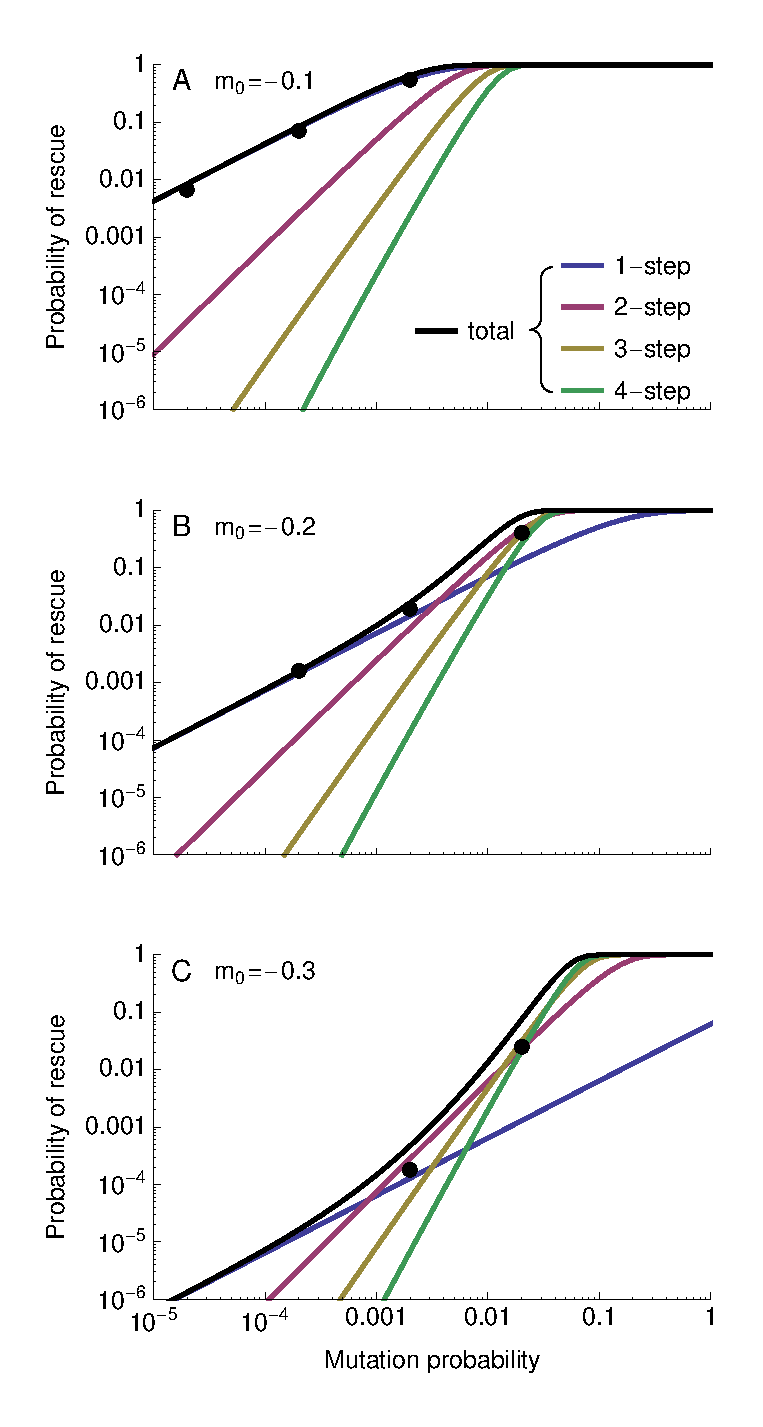
\includegraphics[width=\linewidth]{FigureS1.eps}
\caption{
The probability of rescue as a function of mutation rate for three different levels of initial maladaptation.
See Figure 3 for details.
Other parameters: $n=4$, $\lambda=0.005$, $m_{max}=0.5$, $N_0=10^4$.
}%
\label{fig:1vs2U}
\end{figure}
%%%%%%%%%%%%%%%%%%%%%%%%%%%%%%%%%%%%%%%%%%%%%%%%%%%

%%%%%%%%%%%%%%%%%%%%%%%%%%%%%%%%%%%%%%%%%%%%%%%%%%%
\begin{figure}[htbp]
\centering
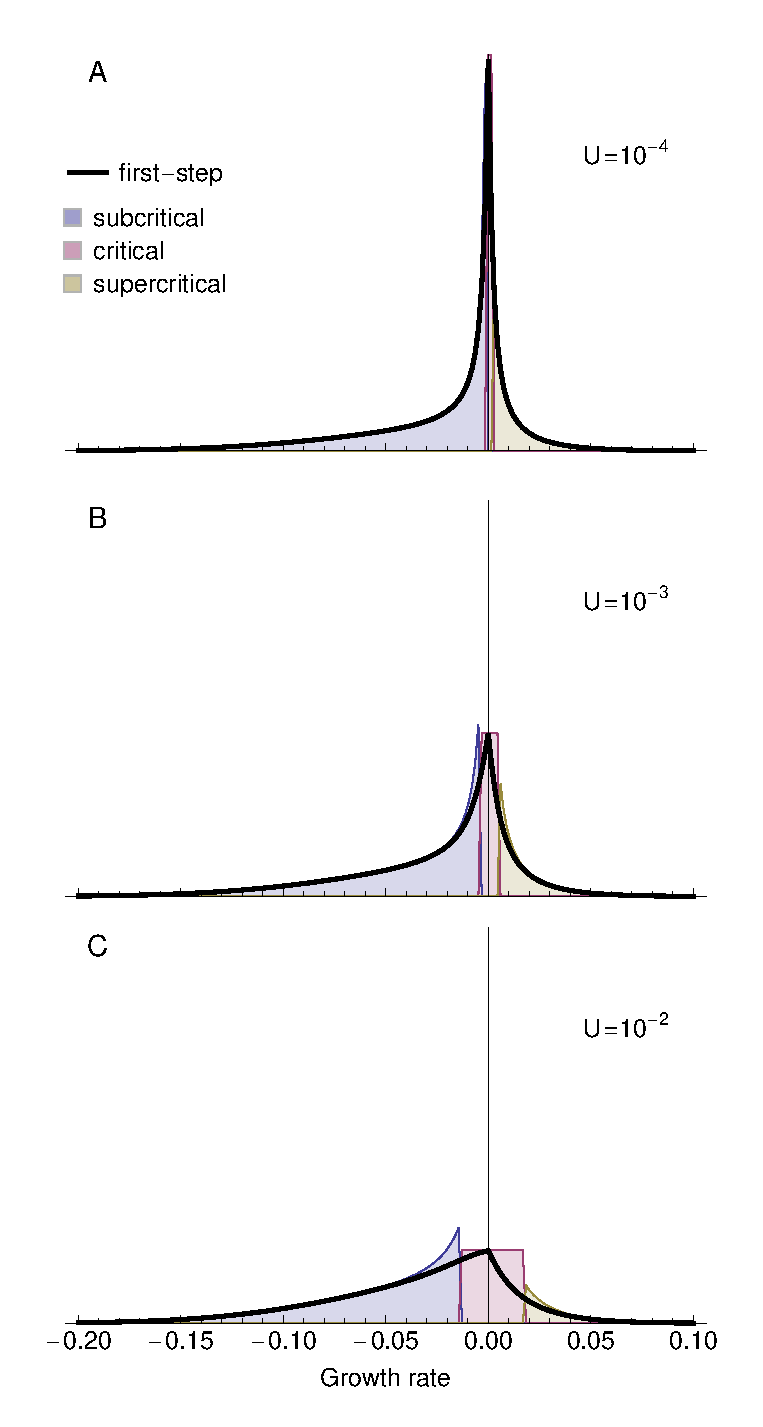
\includegraphics[width=\linewidth]{FigureS2.eps}
\caption{
The distribution of first-step mutant growth rates given 2-step rescue under three mutation rates. 
See Figure 7 for details.
Parameters: $n=4$, $\lambda=0.005$, $m_{max}=0.5$, $m_0=-0.2$.
}%
\label{fig:firststepDFE_mutation}
\end{figure}
%%%%%%%%%%%%%%%%%%%%%%%%%%%%%%%%%%%%%%%%%%%%%%%%%%%

%%%%%%%%%%%%%%%%%%%%%%%%%%%%%%%%%%%%%%%%%%%%%%%%%%%
\begin{figure}[htbp]
\centering
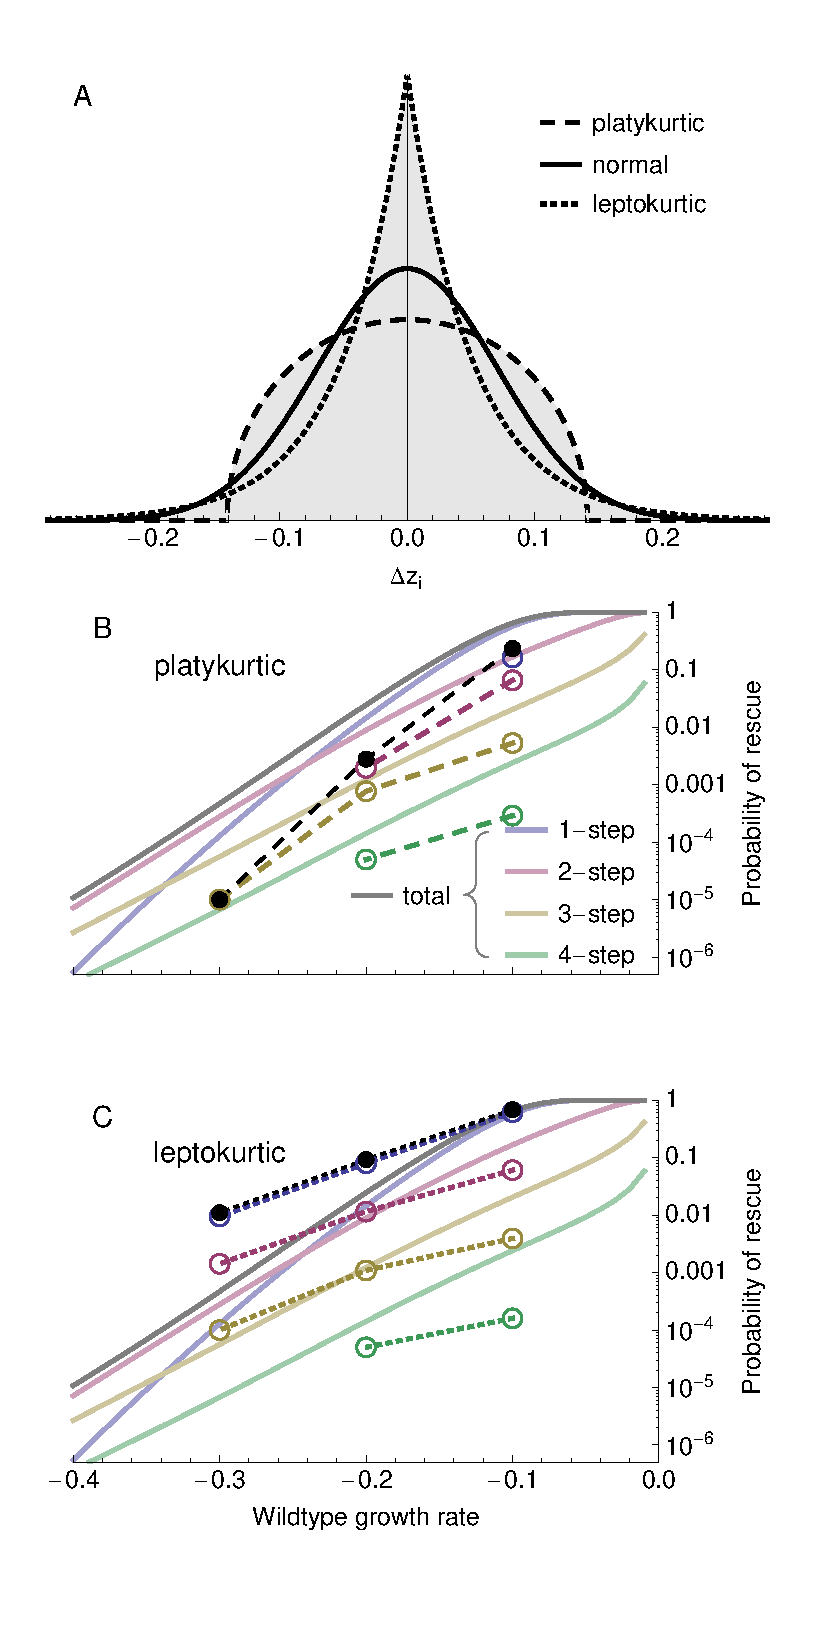
\includegraphics[width=\linewidth]{FigureS3.eps}
\caption{
(\textbf{A}) One-dimensional slices of multidimensional platykurtic (dashed; semicircle), normal (solid; as used in main text), and leptokurtic (dotted; Laplace) mutational distributions with the same (co)variance but varying kurtosis.
(\textbf{B},\textbf{C}) The probability of 1-, 2-, 3-, or 4-step rescue with platykurtic and leptokurtic mutational distributions, respectively.
The dots and broken lines represent simulation results ($10^5$ replicates for each wildtype growth rate).
The solid lines are the numerical results for the normal mutational distribution (as in Figure 3).
Parameters: $N_0=10^4$, $U=2\times 10^{-3}$, $n=4$, $\lambda=0.005$, $m_{max}=0.5$.
}%
\label{fig:lepto_platy_prob}
\end{figure}
%%%%%%%%%%%%%%%%%%%%%%%%%%%%%%%%%%%%%%%%%%%%%%%%%%%

%%%%%%%%%%%%%%%%%%%%%%%%%%%%%%%%%%%%%%%%%%%%%%%%%%%
\begin{figure}[htbp]
\centering
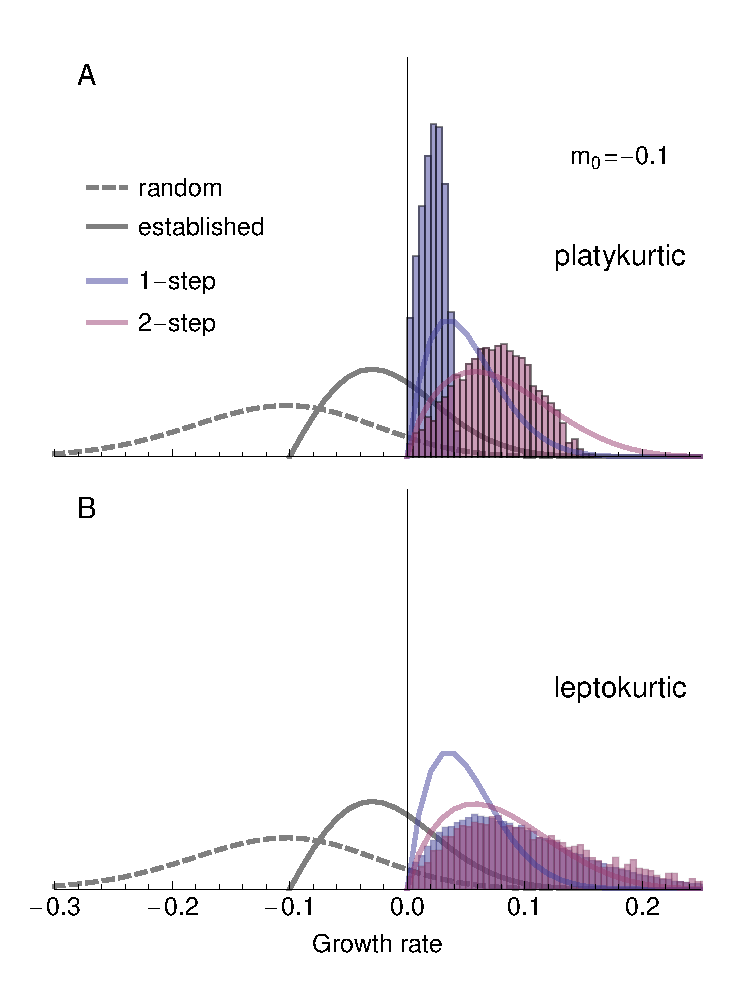
\includegraphics[width=\linewidth]{FigureS4.pdf}
\caption{
The distribution of growth rates among rescue genotypes under 1-step (blue) and 2-step (red) rescue with (\textbf{A}) platykurtic and (\textbf{B}) leptokurtic mutational distributions (see Figure \ref{fig:lepto_platy_prob}A).
The solid lines are predictions for a normal mutational distribution (as in Figure 6).
The histograms show the distribution of growth rates among rescue genotypes observed across $10^5$ replicate simulations.
Parameters: $N_0=10^4$, $U=2\times 10^{-3}$, $n=4$, $\lambda=0.005$, $m_{max}=0.5$, $m_0=-0.1$.
}%
\label{fig:lepto_platy_dfe}
\end{figure}
%%%%%%%%%%%%%%%%%%%%%%%%%%%%%%%%%%%%%%%%%%%%%%%%%%%

%%%%%%%%%%%%%%%%%%%%%%%%%%%%%%%%%%%%%%%%%%%%%%%%%%%
\begin{figure}[htbp]
\centering
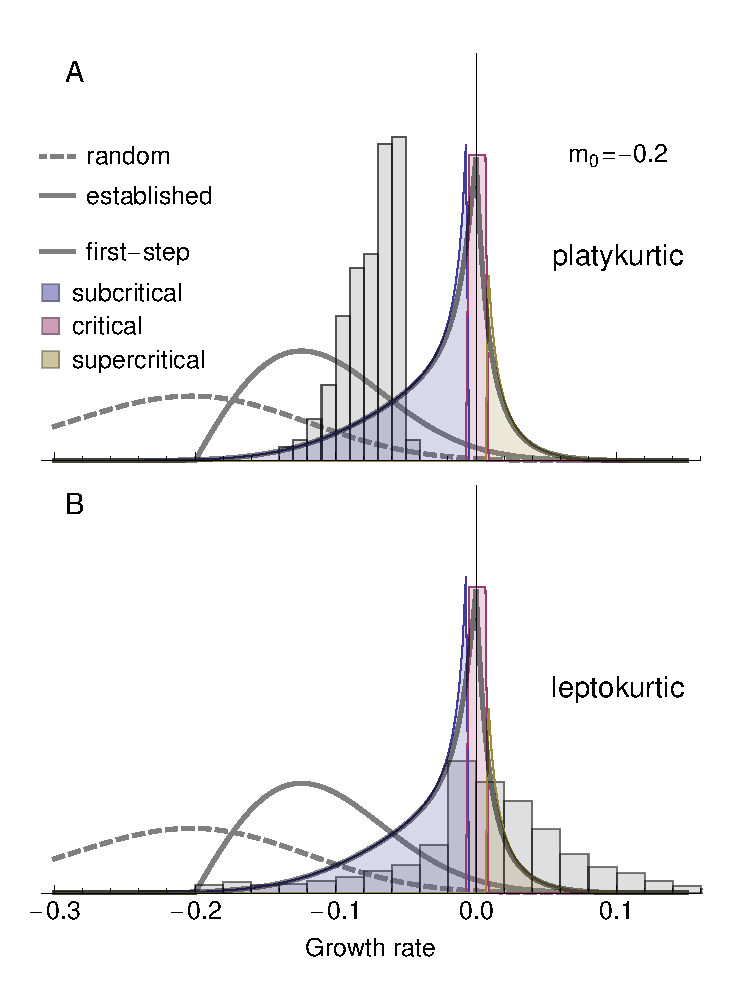
\includegraphics[width=\linewidth]{FigureS5.pdf}
\caption{
The distribution of growth rates among first-step mutations that lead to 2-step rescue with (\textbf{A}) platykurtic and (\textbf{B}) leptokurtic mutational distributions (see Figure \ref{fig:lepto_platy_prob}A).
The curves and shadings are predictions for a normal mutational distribution (as in Figure 7).
The histograms show the distribution of growth rates observed across $10^5$ replicate simulations.
Parameters: $N_0=10^4$, $U=2\times 10^{-3}$, $n=4$, $\lambda=0.005$, $m_{max}=0.5$, $m_0=-0.2$.
}%
\label{fig:lepto_platy_dfe_int}
\end{figure}
%%%%%%%%%%%%%%%%%%%%%%%%%%%%%%%%%%%%%%%%%%%%%%%%%%%

%%%%%%%%%%%%%%%%%%%%%%%%%%%%%%%%%%%%%%%%%%%%%%%%%%%
\begin{figure}[htbp]
\centering
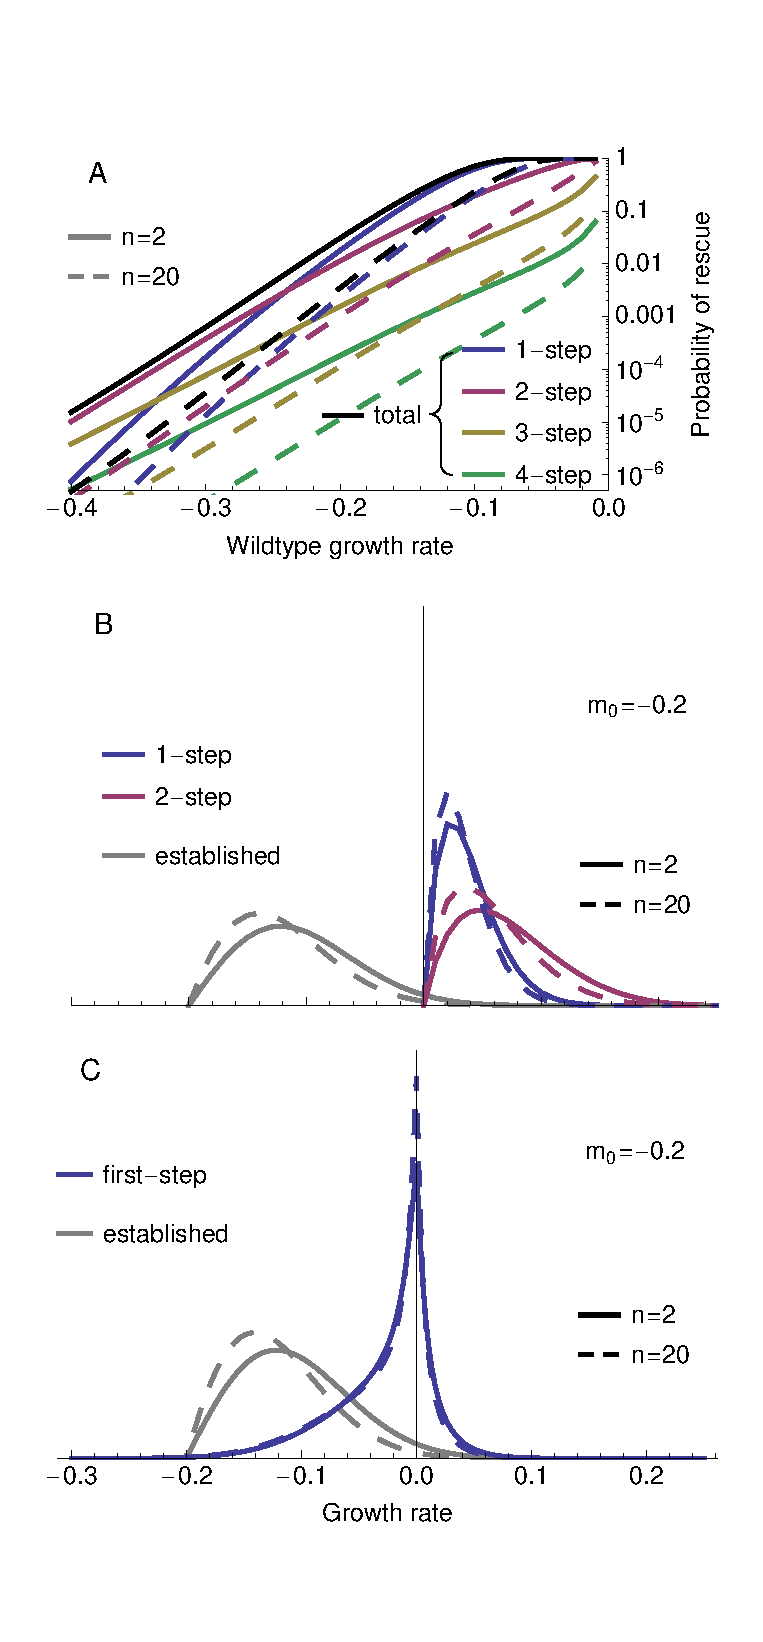
\includegraphics[width=\linewidth]{FigureS6.eps}
\caption{
The effect of the number of phenotypic dimensions, $n$, on (\textbf{A}) the probability of $k$-step rescue, (\textbf{B}) the distribution of growth rates among rescue genotypes, and (\textbf{C}) the distribution of growth rates among first-step mutants that lead to 2-step rescue.
Curves are numerical results, as in Figures 3, 6, and 7.
Parameters: $N_0=10^4$, $U=2\times 10^{-3}$, $\lambda=0.005$, $m_{max}=0.5$.
}%
\label{fig:dimension}
\end{figure}
%%%%%%%%%%%%%%%%%%%%%%%%%%%%%%%%%%%%%%%%%%%%%%%%%%%

\end{document}